% Template for PLoS
% Version 1.0 January 2009
%
% To compile to pdf, run:
% latex plos.template
% bibtex plos.template
% latex plos.template
% latex plos.template
% dvipdf plos.template

\documentclass[10pt]{article}

% amsmath package, useful for mathematical formulas
\usepackage{amsmath}
% amssymb package, useful for mathematical symbols
\usepackage{amssymb}

% graphicx package, useful for including eps and pdf graphics
% include graphics with the command \includegraphics
\usepackage{graphicx}

% cite package, to clean up citations in the main text. Do not remove.
\usepackage{cite}

\usepackage{color} 

% Use doublespacing - comment out for single spacing
%\usepackage{setspace} 
%\doublespacing


% Text layout
\topmargin 0.0cm
\oddsidemargin 0.5cm
\evensidemargin 0.5cm
\textwidth 16cm 
\textheight 21cm

% Bold the 'Figure #' in the caption and separate it with a period
% Captions will be left justified
\usepackage[labelfont=bf,labelsep=period,justification=raggedright]{caption}

% Use the PLoS provided bibtex style
\bibliographystyle{plos2009}

% Remove brackets from numbering in List of References
\makeatletter
\renewcommand{\@biblabel}[1]{\quad#1.}
\makeatother


% Leave date blank
\date{}

\pagestyle{myheadings}
%% ** EDIT HERE **


%% ** EDIT HERE **
%% PLEASE INCLUDE ALL MACROS BELOW

%% END MACROS SECTION

\begin{document}
\newtheorem{defination}{defination}[section]
\newtheorem{theorem}{theorem}[section]
\newtheorem{lemma}[theorem]{lemma}
\newtheorem{corollary}[theorem]{corollary}
% Title must be 150 characters or less
\begin{flushleft}
{\Large
\textbf{Applying the Random-mixing Scheme to Enhance the Robustness of DHT}
}
% Insert Author names, affiliations and corresponding author email.
\\
Author1$^{1}$, 
Author2$^{2}$, 
Author3$^{3,\ast}$
\\
\bf{1} Author1 Dept/Program/Center, Institution Name, City, State, Country
\\
\bf{2} Author2 Dept/Program/Center, Institution Name, City, State, Country
\\
\bf{3} Author3 Dept/Program/Center, Institution Name, City, State, Country
\\
$\ast$ E-mail: Corresponding author@institute.edu
\end{flushleft}
\tableofcontents
% Please keep the abstract between 250 and 300 words
\section{Abstract}
Distributed hash tables (DHT) are usually used in the open networking environment, where they are vulnerable to the Sybil attacks. To enhance the robustness of the system, the random-mixing (RM) scheme is harnessed to handle the Sybil attacks in the paper. The new coming node must ask the Certificate Authority (CA) for its signature and certificate. The certificate which records a RM joining process completely affirms the validity of the node. To prevent the adversary from accumulating identifiers, with the help of the substituting property in the RM joining process, the node makes use of the latest certificates to judge the legality of another identifier. The analysis is carried out in detail on the number of the certificates which are needed to store in every node, and the asymptotic solution of this problem is given. The analysis and simulations show that the mean certificates stored in each node are  , where n is the size of the network.
% Please keep the Author Summary between 150 and 200 words
% Use first person. PLoS ONE authors please skip this step. 
% Author Summary not valid for PLoS ONE submissions.   
\section{Author Summary}

\section{Introduction}
Because of its high scalability,DHT\cite{ref1,ref2,ref3,ref4} won the people’s attention. But for actual deployment of DHT, scalability is just one aspect of factors to consider, and system security is another problem that cannot be avoided. \\
  Traditional Security mainly focus: information integrity, tamper-resistance, non-repudiation; in DHT applications, concerns are somewhat different. In general, because the DHT algorithm itself has a certain amount of redundancy, random attacks on the network will not cause great damage. However, if the adversaries can obtain a large number of ID numbers, using these ID numbers attacking DHT network which can cause the loss of DHT network redundancy advantages, this is called Sybil attack. Douceur[5] believes the DHT security issues to consider is how to distinguish between the different entities. To do this, either ensure every node can directly to verify, or the presence of a certification authority (CA) to confirm the identity of the other nodes. Because of the method of directly verifying nodes has poor scalability, so usually there is an explicit or implicit CA, such as in CFS[6], the node ID is the hash value of the IP address; and EMBASSY[7] takes advantage of the encryption key of hardware.\\
    Sybil attack poses a dilemma for design choices of DHT system:either maintain the system openness, newcomers can more easily access the network; or raise the barriers to entry, enhancing the security of the system. Can we get better about a compromise between the two? In this paper’s opinion, random mixing (RM) algorithm which is proposed by Scheideler[8] and Awebuch[9] , or Cuckoo algorithm[9] can be able to do this.\\
    RM algorithm is that: Place black and white stones in a ring, white stone for honest node, black stone for attack nodes. Assuming that all nodes are controlled by an adversary, and the adversary has two options:either places in the ring with a black stone, or get any black stone out of the ring. In this game, placing stones must follow the K rounds replacement rules:1st round,new stone randomly selects a location to replace the stone on the location;the replaced stone randomly replaces another stone in the ring in 2nd round; K-round,the stone which is replaced in last round should be randomly inserted into the ring.\\
    In this game, Scheideler[8] proved that:when \(k=3\)  ,if the adversary controls no more than $\frac{1}{4}$ of the total black stone, then in the continuous \(\Theta(log n) \) stones,white stone can be in the majority with high probability. This paper believes that, when network scale is big, this conditin is easy to be satisfied. But in the practical application of the RM algorithm, the adversary will do every possible to destroy K rounds replacement rules to place attack nodes to his desired position, so there must be some means of ensure K rounds replacement rules will be carried out. To solve this problem, this paper uses an explicit CA to authenticate K rounds replacement process, which guarantees that the adversary can not forge the ID number and guarantees ID can be verified. Further, to prevent an adversary cumulates ID numbers, we use recent certificate to determine whether an ID has expired or not, so this put an end to the attempt that adversary illegally joins to the network by network maintenance agreement. \\
    Later is organized as follows, section 2 does a brief review of related work; section 3 gives the node join algorithm based on RM, and discusses how a node uses the certificate to determine whether the ID is expired; section 4 take a theoretical analysis on algorithm practicality;section 5 verifies theoretical results through simulation experiments;finally conclude and give some results.
\section{Related Work}
Security of DHT has been considered at the beginning of the algorithm's design, Castro[10] has consideration for four aspects of security:security for allocation of node ID, security for maintaining of the routing table, security for message forwarding, and security for data. Among them, security for allocation of node ID is the foundation of the remaining three ones. In the preventive measures proposed by Castro, node must pay for the ID or bind the node ID to the identity in the real world., but to do so will undoubtedly limit the applications of the DHT algorithm.\\
The term of the Sybil attack was first defined by Douceur[5], Douceur thinks if you can not distinguish the identity of the remote node through explicit or implicit CA, a large part of the system will be mastered by adversary. And, to a system relied on the implicit CA, it must be clear that how secure such implicit CA can provide. For example, the IPv6 protocol, you can easily get a lot of IP address; so implicitly CA which dependent on the IP address bound does not provide sufficient security guarantees for the system.\\
Yu [11] in  SybilGuard algorithm, try to use social degree of access in real word to distinguish the identity of a remote user, and believe the connection between honest node set and rival node set has small cut. Yu and so on use Random-Walk algorithm to find this cut. SybilGuard algorithm is suitable for unstructured P2P networks.\\
In DHT algorithm,before new node enter the network, we usually need to know an online node, which depend this online nodes' introduction to enter the network. According to this bootstrap relations, nodes in the network make up a bootstrap tree; the closer to the root node, the higher probability that it is the honest node. Danezis[12] used this phenomenon and presents measurements to maintain the routing performance under the Sybil attack, this algorithm is more suitable for the hierarchical structure of the DHT network.\\
Thoughts of Bazi[13] is more fundamental, he studied how to use network measurements to screen the remote entity. Lighthouse, consists of a series of CA nodes, measured the screening entities, according to the triangle inequality, this measurement value has the lower limit. Unfortunately these algorithms are to be further developed.\\
Rowaihy[14] tried to build an hierarchical adaptive nodes management system in the DHT network. In this system,  leaf nodes want to be raised as the management nodes ( the internal nodes of the tree ),and must answer the children nodes' problem(puzzles). These problems will take a lot of computing resources, this increases adversary's difficulty of controlling other nodes, but at the same time it will cause a lot of waste of computing resources. \\
Fireflies[15] is a funny design. In Fireflies,Network topology is made up with \(2t+1\) Chord rings, each physical node joins the  \(2t+1\)-dimensional network at the same time. Each node's \(2t+1\) precursors make up the arbitration set for this node, while the introduction of the accusation/rebuttal mechanism to regulate the behaviors of nodes.\\
Condie[16] presented a solution, which is very close to RM and Cuckoo rules. This scheme uses random numbers server as the CA, the random numbers server cycles to generate random numbers, while the node ID is a function of the random number.  After every period of time, node IDs will change, therefore, the locations of the nodes have a random change. Since the node ID can not be predicted, and can be verified; therefore, the adversary can not pre-select ID,also can not accumulate ID, honest nodes and attack nodes can be uniformly mixed. Disadvantage of this solution is: the network is changed frequently, therefore it is not suitable for the occasion of the storage service.\\
Similar to RM[8],The rules of Cuckoo[9] uses the replacement operation, when new node is joined, it was asked to replace the nodes within the \(c\log{n}/n\) distance, the nodes replaced then will be re-inserted into the network.  Awerbuch and Scheideler proved that,under Cuckoo rules,the normal nodes and the attack nodes are evenly mixed with high probability. Compared to RM, the rule of Cuckoo also has the advantage of load balancing. This paper believes,load balancing of DHT and Sybil attacks are two orthogonal issues, we can use other measurements to compensate for the lack of RM programs; and the proposed scheme is also applicable to the Cuckoo rules.\\
Based on RM, Fiat[17] import the Byzantine to handle the cheating of adversary. Actually, this design is complete, which not only solve the sybil attack, but also be able to handle routing security and data security issuses. However, the cost the this proposal is expensive. If it is tolerableness to afford the cost when join some nodes. However, it is not affordable if every message must be verified by the arbitration set. \\
Similar with the design of Fiat, King[18] proposed a security algorithm based on Byzantine protocol and leader selection protocol. However, the cost of this algorithm limits the application of this algorithm.
\section{Algorithm Discription}
Without loss of generality, this paper select Chord[1] network as the basic model, and we discuess the application based on RM. Limited to the length of this article, we omits the Chord network.\\
\subsection{ID Generation scheme}
To defense the Sybil attack, the first problem to handle is to provide a secure ID generation scheme. If the adversary can able to select ID, then he can attack in a good position. So you must deprive him of the ability to select position in address space or limit the space the adversary can use. The RM algorithm make all nodes mixed uniformly by random-mixing. This actually limit sthe space the adversary can select, while the former one corresponds to the secure ID generation scheme.\\
One secure ID generation scheme has several meanings: firstly, the ID can not be forged. This is very to be understood. If the adversary can forge ID, that means he was able to arbitrarily select a random position, which will further undermine the security of DHT. Secondly the ID should be verifiable, this actually is the reflection of the first meaning.  How to determine whether the node is a forged node? This requires that the node ID is self-validation(self-verified). The last meaning of it is subtle, requiring the application of one node should be constantly changing, over time. If one node can get the same ID, then the adversary can receive a lot of ID by different identities, and choose some ID from these which him in better position. For example, the adversaries can  use different IPv6 addresses, and registers a lot of ID, then select a good position. This is called adaptive joined attack[9]. Therefore, the last meaning actually make the selection range of the adversaries constantly changing overtime. \\
The ID generation scheme use the explicit CA. Let's assume that every node has pairs of keys \(K^+\) and \(K_-\). where \(K^+\) represents the public key,  and \(K^-\) represents the private key. And define the cryptographic  operation as \(E[x,k]\). Which represents we use plaintext \(x\) is encrypted into ciphertext by the key \(k\). When each node joins the network, you must collect signatures from CA, and the signature is defined as \(sig(p)=E[K^+||T,K^-(u)]\), where \(K^+\) is the public key of \(p\), and \(T\) is the timestamp,\(||\) represents the  string concatenation operator, and \(K^-(u)\)is the private key of node \(u\) in CA. The node ID is defined as the hash value of signature \\
In this scheme,  unless the private key of CA is intercepted, otherwise  it is difficult to forge a node ID. Let's assume that the public key \(K^+(u)\) of node u in CA are sent to other nodes by some out-of-band or Key exchange protocol(IKE). When one node \(p\), shows his signature, other nodes first use the public key \(K^+(u)\) of CA to verify the signature of this node; then use the hash function to calculate the node ID. Finally, since the signature contains timestamps, which makes the signature differs in one node varies over time. So the adversary can not predicate the signature and changes of IDs.
\subsection{K-round Joining Replacement}
Based on the generation scheme of the security ID, this section will apply the algorithm of RM.  The core part to apply the k-wheel replacing rules is to make sure the K-round replacement is enforced.  All it needs to do is to use the Byzantine protocol. But due to the relatively large overhead of the Byzantine agreement, this paper uses an explicit CA to carry out the k-round replacing rules. CA not only provide a signature verification but also grant certificate of k-round replacing for the node to join the network. The certification completely record the process of the k-round replacing. Only both the signature and certification are verified, its neighbor nodes then make connection to the joining node itself.\\
Let's assume the process of the k-round replacement: In 1st round, the new node a substitute the direct successor b of a. In 2nd round, node b is granted a new position \(b'\), and \(b'\) subsited its direct successor c. In 3rd round, the node c is granted a new position \(c'\), then directly insert into the new position \(c'\). The certification in this k round represents below:
\begin{equation}
    cert=E[sig(a)||sig(b)||sig(b')||sig(c)||sig(c')||T,K^-(u)]
\end{equation}
Where $sig(a)$ is the sigature of a,$sig(b)$ is the old signature of node b, and $sig(b')$ is the new signature of node b.T is the timestamp when the certification created. Meanwhile, we defines the neighbours of the nodes in address space $[p-c\ln{n},p+c\ln{n}]$, where n represents the number of online nodes.  With these prepared, we just describe the K-round Joining Replacement algorithm.\\
\begin{center}
    Algorithm 1. The K-round Joining Replacement
\end{center}
\begin{minipage}[l]{360pt}
a is a new node, u is one CA node\\
J1. a  swap public key with u , and request to join the network\\
J2. u calculate the signature and ID of a , then find the direct successor of a .\\
J3. u swap public key with b, and calculate the new signature of b and new ID number b'.\\
J4. u find the direct successor of b' .\\
J5. u swap public key with c , calculate the new signature of c and the ID number c' and the K-round Joining Replacement certification.\\
J6. u send new signature and certification to a,b,c.\\
\end{minipage}
This paper assume the communication between the nodes first need to exchange public key through IKE. Subsequent communication message use hash function to calculate abstract and then use private key to encrypt the abstract. The ciphertext of abstract is attached to the messages.\\
Algorithm 1 follows the k-round replacing design, and the result of algorithm is that the nodes   gain the $a,b,c$ new signature and certification. The old and new position of the nodes $a,b,c$ are not predictable. \\
In step J3 and J5 of algorithm 1, if the node $b$ or $c$ refuses to interact with IKE. Then node $u$ directly regard $b$ and $c$ as offline nodes, and use the next successor as the direct successor. By using the node validation algorithm discussed later ,  the nodes which reject to interact with IKE will be the illegal nodes, and the protocol for maintain protocol will delete all these nodes.\\
The steps which can be attacked are step J2 and J4. The nodes $u$ found probably not the direct successor node.To prevent this,$u$ can continuously ask their neighbors to get the real successor nearby the position of node $a$ and node $b$, and public the new replacement certificate and the forged node will be kicked out.  
\subsection{ID Validation}
After running the algorithm 1, new joined nodes and replaced nodes can gain the new signature and certification,  and these nodes doesn't really appear in the network topology. Only when the protocol of maintaining the topology become stabilize, other nodes can set up connection with them.\\
Although the adversary cannot be forge signature and ID, he still can accumulate a lot of signature sand certifications. Most of these accumulated IDs are replaced in K-rounds replacement.   If the adversary use these replaced ID to join the network through the topology maintenance protocol, he can probably destroys the K-round replacement rule. So we must find a method to patch this hole.\\
If the neighbour nodes save all previous certifications, and all adversaries try to join the network again by using the replaced ID, the neighbour nodes then can penetrate the attempts of adversaries, and be able to patch this hole. But it is unrealistic to completely save all old certifications. Are there other ways existed, which can significantly reduce the number of certification need to save. \\
Noting that in algorithm 1, the node replaced by node $a$ is its the direct successor $b$.So there are no online nodes existed in range $(a,b)$. Similarly, there are no online nodes existed in range $(b',c)$. This paper assumes that $(a,b)$ and $(b',c)$ are replacement intervals. When adversaries want to let the node $e\in(a,b)$ join the network, then node a and its neighbour node can use the certifications it contained to infer that $e$ is a expired ID and refuse $e$'s request to join the network.\\
Based on this idea, In this paper, the recent certifications are saved on neighbour nodes to verify whether some IDs are expired. Further, how many certifications need to be saved by the neighbour nodes? If the replacement intervals of the certifications can completely cover the neighbour area $[p-c\ln{n},p+c\ln{n}]$. Then the old certifications are not necessary to be saved. Thus the minimum number of recent certifications to cover the complete neighbour region will be enough.\\
To set up database S and save all recent certifications in every node, it it required that the replacement of the recent certifications can completely cover the neighbour range.  The algorithm 2 is running on nodes to verify whether one ID is expired.\\
\begin{center}
Algorithm 2.AlgorithmID Validation algorithm 
\end{center}
\begin{minipage}[l]{360pt}
    S is the database certification,$id$ is one node need to be verifed,its certification is $cert$ \\  
    L1. If $id$ is not in the range of neighbours,directly return illegal;\\
    L2. If S contain one certification, and it is newer than $cert$,and $id$ is within the range of its replacement, then the $id$ is illegal;\\
    L3. Otherwise accept $id$, mark it as legal,and insert $cert$ into S.
\end{minipage}
In algorithm 2, first we need to check whether the id is within the neighbour range, if it is not within the neighbour range, we mark it as illegal id. If the database certification contains some certification and it can cover this id, and the timestamp of certification in the database is newer, then mark mark this id illegal.  The logical branch of L3 in algorithm 2 contains: (1) $cert$ is newer than other certifications in S. (2)$id$ is not covered by S. The logical branch (1) corresponds to the new certification. While (2) probably because the certifications in database S can not completely cover the whole neighbour range. \\
Nodes need to exchange information in database S regularly. If the time stamp of the received certification updates, we insert this certification into database S. If the new inserted certification's replacement interval covers the replacement interval of old ones, just delete the old certifications. In practical application, if one node of the neighbour nodes is honest, the completely certification database can be able to inherited.\\
By using the ID validation algorithm, when the protocol of topology maintenance become stabilize, we can verify whether one node is legal or not. We just neglect the request of illegal nodes, then the illegal nodes will be killed out of the network. This paper omits the description of the modified stabilize algorithm. 
\section{Performance Analysis}
In algorithm 2, we use the recent certifications saved on database S to verify whether on ID is legal, which require the certification's covered interval is able to cover the neighbour intervals. Compared with the old method which stored all certifications.  The certification numbers in algorithm 2 is much less. However, the number of certifications we need to save is still huge, then the RM application scheme proposed in this paper is not practical. In this section, we make some theoretical analysis on this problem\\
We use another presentation to describe the considered problem: how many certifications I need to completely cover the network address space? If the replacement interval can be seen as segments, this convert it into a circle covering problem.  Fellow[19] make a conclusion about how to use equal-length segments to cover the circle. But the problem here is not suitable for it. The length of cover segments(replacement intervals) is variable. Fortunately, there are so many mathematicians try to solve how to use random-length segments to cover the circle. Siegel[20] and Domb[21] use different methods to solve this problem. In this paper, we use the Domb method.\\
First we presents the conclusion of Domb. Let's assume that $P(l)$ is the probability for a circular arc with length $l$ to be covered. We defines the initial probability as $P_0(l)$, which represents the probability of the segment covers the whole arc,whose starting point is just before the circle arc, Meanwhile introduce the intermediate function $v(l)$, defined as (7).Then let's assume the distribution density of cover segment is $u(l)$. The probability of the random segments to be covered:
\begin{equation}
    P(l)=\int_{0}^{l} v(x)P(l-x)dx+P_0(l)
\end{equation}
Since (2) is just a convolution of $P(l)$, we then transform formula (2) by using Laplace's transformation , then we get:
\begin{equation}
    P(s)=\frac{P_0(s)}{1-V(s)}
\end{equation}
Next, this paper apply formula(2) and formula(3) to solve problems. First we introduce two lemmas. Limited to the length of paragraph, this paper omits the proof the two lemmas. 
\subsection{Two Lemmas}
In a unit circle with length 1, we randomly insert   nodes, the interval between nodes and the probability of the number of nodes that appears on one arc obeys the following distribution: 
\begin{lemma}
    If the nodes randomly select ID in address space, then the node interval obeys negative exponential distribution,$P(l)=1-e^{-\alpha{l}}$
\end{lemma}
\begin{lemma}
    If nodes in address space randomly select one ID. Then for one contiguous address space, the nodes obey the Poisson distribution,$P(k)=\frac{(\alpha{l})^k}{k!}e^{-\alpha{l}}$
\end{lemma}
 The length of the replacement interval is one random variable, according to lemma 1,  it obeys the negative exponential distribution with parameter $n$, where n is the network size. Thus the distribution density and CDF of replacement interval are respectively $u(l)=ne^{-nl}$, and $U(l)=1-e^{-nl}$. Assume the number of total cover segments is $\lambda$, and the clockwise direction is the positive direction. According to lemma 1, the starting location of every cover segment obeys the negative exponential distribution with parameter $\lambda$.
 \subsection{The Initial Distribution}
 According to lemma 2, calculate the initial distribution $P_0(l)$.
 \begin{equation}
    P_0(l)=\int _{0}^{1-l}\lambda{dx}\int _{l+x}^{1}u(y)dy
 \end{equation}
 In formula(4),$e_{-\lambda{l+x}}$ represents there are no cover segments in $(l+x)$, and $\lambda{dx}$ represents there is one cover segment starting point on  differential element $dx$. And $\int _{l+x}^{1}u(y)dy$ represents the sum length of cover segments that exceed $(l+x)$. Since the cover segments distributed in interval $[0,1)$, so the  integral limit of $x$ is from $0$ to $(1-l)$.  The formula (4) can be deduced as: 
\begin{equation}
    P_0(l)=\frac{\lambda}{\lambda{+n}}e^{-(\lambda{l}+n)}+\frac{n}{\lambda{+n}}e^{-(\lambda{+n})}
\end{equation}
According to formula(5), when $l\to \infty$,$P_0(l)$ converged to $\frac{n}{\lambda{+n}}e^{-(\lambda{+n})}$. Use Laplace's transformation on $P_0(l)$ with $0<l\leq{1}$, then we get:
\begin{equation}
    P_0(s)=\frac{\lambda (1-e^{-(s+\lambda +n)})}{(s+\lambda +n)(\lambda +n)}-\frac{e^{-n}-e^{-(s+\lambda+n)}}{s+\lambda }+\frac{n(e^{-(\lambda +n)}-e^{-(s+\lambda +n)})}{(\lambda +n)s}
\end{equation}
\subsection{Intermediate function}
The Intermediate function $v(l)$ is defined as:
\begin{equation}
    v(l)=\lambda e^{-\lambda l}[1-U(l)]e^{\lambda \int _{0}^{l}U(x)dx}
\end{equation}
Substitude it into the cover segement U(l):
\begin{equation}
    v(l)=\lambda e^{-nl-\frac{\lambda}{n}+\frac{\lambda}{n}e^{-nl}}
\end{equation}
Make Laplace's transformation on $v(l)$.
\begin{equation}
    V(s)=\int _{0}^{\infty}e^{-sl}\lambda e^{-nl-\frac{\lambda}{n}+\frac{\lambda}{n}e^{-nl}}dl=\lambda e^{-\frac{\lambda}{n}}\int _{0}^{\infty}e^{-(s+n)l}e^{\frac{\lambda}{n}e^{-nl}}dl
\end{equation}
According to formula (9),$V(s)$ exists. Since the solution of $1-V(s)=0$ is the pole of (3). And the position of pole can direct affect time-domain properties. So we must take the detailed understanding of $V(s)$. \\
Limited to the length of the paper, we omit the detailed analysis of $V(s)$. Though analysis,$1-V(s)=0$ only has solutions in the real axis. While $s\in R$,$V(s)$ is a monotone decreasing function.$V(0)=1-e{-\frac{\lambda}{n}}$ $0<V(0)<1$. When $0\to \infty$, then $V(s)\to 0$. Thus the solutions of $1-V(s)=0$ is on negative real axis. Let's assume the solution is $-\gamma$.
\subsection{Cover Probability}
Substitue the formula (6) and (9) into formula (3), we get:
\begin{equation}
    P(s)=\frac{\frac{\lambda (1-e^{-(s+\lambda +n)})}{(s+\lambda +n)(\lambda +n)}-\frac{e^{-n}(1-e^{-(s+\lambda)})}{s+\lambda }+\frac{ne^{-(\lambda +n)}(1-e^{-s})}{(\lambda +n)s}}{1-\lambda e^{-\frac{\lambda}{n}}\int_{0}^{\infty}e^{-(s+n)l}e^{\frac{\lambda}{n}e^{-nl}}dl}
\end{equation}
According to the complex form of formula(10), here we just consider its approximate solution. For a Laplace transformation, its pole position decides the time-domain transition process.In formula (10), there are four  possible positions for pole.$-\lambda , -\lambda ,-n,0,-\gamma$. Since $n$ is the network size,$\lambda$ is the number of segments cover segments. Thus $\lambda>n$. Considered the formula (10), the coefficients of pole $-\lambda$ and 0 are all very small, these two poles can be neglected. Thus:
\begin{equation}
    P(s)\approx \frac{\frac{\lambda (1-e^{-(s+\lambda +n)})}{(s+\lambda +n)(\lambda +n)}}{1-\lambda e^{-\frac{\lambda}{n}}\int _{0}^{\infty}e^{-(s+n)l}e^{\frac{\lambda}{n}e^{-nl}}dl}
\end{equation}
In order to further get the approximate value(11), by using the Domb conclusion, when $l\gg \frac{1}{n}$,$\frac{1}{n}$ is the average value of cover segments. So you can approximately regard $V(s)$ as one intermediate function by using equal segments $\frac{1}{n}$ to cover the circle. This approximate intermediate function is [21]: 
\begin{equation}
    \widetilde{A}(s)=\frac{\lambda}{s+\lambda }(1-e^{-\frac{s+\lambda }{n}})
\end{equation}
Let $s+\lambda e^{-\frac{s+\lambda }{n}}=0$ , the solution of $s\in R$ is $\widetilde{\gamma}$. Where $\widetilde{\gamma}=-nW(-\frac{\lambda}{n}e^{-\frac{\lambda}{n}})$, And $W(x)=xe^{x}$ is the  Lambert-W function[22].
\begin{equation}
    P(s)\approx \frac{\lambda (s+\lambda )(1-e^{-(s+\lambda +n)})}{(\lambda +n)(s+\lambda +n)(s+\widetilde{\gamma})}
\end{equation}
To expand the formula (13), we get:
\begin{equation}
    P(s)\approx \frac{\lambda (s+\lambda)}{(\lambda +n)(s+\lambda +n)(s+\widetilde{\gamma})}=\frac{\lambda}{\lambda +n}\lbrack \frac{A}{s+\lambda +n}+\frac{B}{s+\widetilde{\gamma}} \rbrack (1-e^{-(s+\lambda +n)})
\end{equation}
\[A=\frac{n}{\lambda +n-\widetilde{\gamma}},B=\frac{\lambda-\widetilde{\gamma}}{\lambda +n-\widetilde{\gamma}}\]
To make Laplace Transform Inversion on formula (14). 
\begin{equation}
    P(l)\approx \frac{\lambda}{\lambda+n} \lbrack Ae^{-(\lambda +n)l}+Be^{-\widetilde{\gamma}l} \rbrack-\frac{\lambda}{\lambda +n}e^{-(\lambda +n)} \lbrack Ae^{-(\lambda +n)(l-1)}+Be^{-\widetilde{\gamma}(l-1)} \rbrack
\end{equation}
By using the above formula, when $l\to 1$, all others ca be ignored.
\begin{equation}
    P(l)\approx \frac{\lambda (\lambda -\widetilde{\gamma})}{(\lambda +n)(\lambda +n-\widetilde{\gamma})}e^{-l\widetilde{\gamma}}
\end{equation}
Formula (17) is the probability when $l\gg \frac{1}{n}$ and the the circle with length $l$ is covered. The first problem the paper need to consider is the probability when the unit circle is covered. Thus $l=1\gg \frac{1}{n}$. And in algorithm 1, every time when one new node join the network,  one certification will be generated, and the certification contains two replacement intervals, thus $\lambda$ should be multiplied by 2. If let $\delta=\frac{\lambda}{n}$ , we finally will get:
\begin{equation}
    P(1)\approx \frac{4\delta^{2}}{(2\delta +1)^{2}}e^{-\widetilde{\gamma}}
\end{equation}
where $\widetilde{\gamma}=-nW(-2\delta e^{-2\delta})$
\\
\begin{figure}[htbp]
\centering
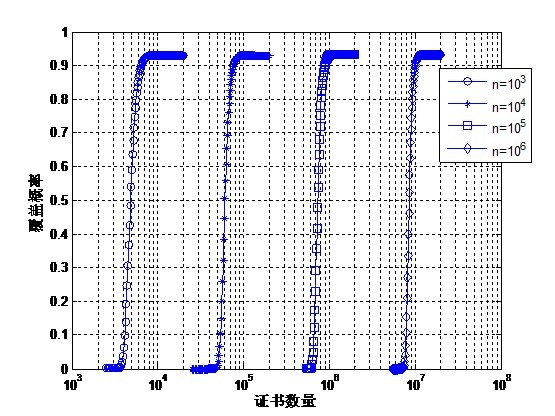
\includegraphics[bb=0 0 440 310,scale=.8]{1.jpg}
\caption{Under different network scale,the probability changes with $\gamma$'s increase}
\label{fig:f1}
\end{figure}\\
If the probability of formula(17) become 0.5, then $4\delta^{2}\approx (2\delta +1)^2$, After solve the formula $e^{-nW(-2\delta e^{-2\delta})}=0.5$ we get:
\begin{equation}
    \delta \approx -\frac{1}{2}Re(W(\frac{0.6931}{n}e^{\frac{0.6931}{n}}))
\end{equation}
where $Re()$ represents the real part, and the function of LambertW just use the range part where smaller then -1. Since $W(x)\approx \ln x- \ln \ln x$, we get :
\begin{equation}
\delta \approx0.1833+1.1513*\lg n
\end{equation}
Since every node need to save the certifications of neighbour, so according the formular (19),  we have the following theorem: 
\begin{theorem}
in this paper's scheme, the number of certifications of nodes is $O (\log ^2 n)$.
\end{theorem}
By using formula (17), when $n=10^3,10^4,10^5,10^6$, the probability of $\gamma$  changes , as shown in Figure 1. In figure 1, you can see that 1) the $\frac{\gamma}{n}$  value of every curve is not big. when $n=10^6$, the $\frac{\gamma}{n}$ value is largest, bigger than 10. While $\frac{\gamma}{n}$  represents the average number of certifications in every node. 2) in some network with size $n$, the probability to completely cover the address space is increased to 0.9 in the smaller $\gamma$, which indicates that the capacity of the certification database S is changing in one narrow range. 3) Noted that the intervals of these four curves are almost the same in logarithmic coordinate, which indicates that with the increasement of the network-size $n$, the increasing amount of $\gamma$ is almost proportion to $\lg{n}$.By using (19) , it is well explained. \\
With the above analysis, the average capacity of certification database library S is not big. For a certain network-size, S is changing in a very narrow range. Considered that every node should kep the certifications of neighbour nodes, the capacity of S is $O(\log ^2{n})$.
\section{Simulation Test}
We use simulation test to verify the analyzed result as follows:
\subsection{Simulation Environment}
In order to program conveniently, this paper selects 32-bit unsigned number as the ID space, and use SHA1 algorithm to generate the random number. At the beginning of the simulation, first we generate n IDs and let them join the network. After the beginning of one experiment, the generated nodes are joined into the network and we random choose one online node and make him leave the network, until all space are covered. \\
 Some caution is needed when the random node selected quit this network, we can not first generate one random ID and then find the ID of direct successors. The distribution is not uniformed with this kind of random quited node selected. \\
 From the results of 5000 times experiments, the range of $\frac{\lambda}{n}$ is within $[4,11]$, and this range is not large. This illustrates that in a network with $n=10000$, the average number of certification to cover the address space $\frac{\lambda}{n}$, is within range $[8c\ln{n},22c\ln{n}]$ on all nodes. This cost is acceptable.
 \subsection{The Distribution of $\frac{\lambda}{n}$ }
 First prove that whether the probability distribution of theory analysis is correct. Check the distribution of the certifications $\lambda$ to completely cover the whole address space. Select network size $n=10000$, and take 5000 rounds tests, then collect the distribution condition of $\frac{\lambda}{n}$.  The test result is shown as Figure 2. The horizontal ordinate is $\frac{\lambda}{n}$. And the vertical coordinate is frequency. \\
 In Figure 2, the probability distribution of (17) can be represented by continuous curve. The simulation result is shown by circles. By observing the Figure 2, you can see that the   simulation result and the result calculated by formula (17) matches well, which indicates that although the deduction of the probability function does a lot of approximate processing. But it has little effect on  the result. We just use (17) to analyze the mean value $\bar{\Lambda}$ of the capacity of the certification database library, and we think it is acceptable.
\subsection{The number of certifications in different network size}
 Next, this paper test the number of certifications to cover the whole address space in different network size. We use different kinds of network size to do the tests, from $n=100$ to $n=1000000$. For the some network size, we take 100 times of tests.\\
 The test result is shown in Figure 3. The horizontal ordinate represents the network size. The vertical coordinates is average number of certifications saved on every node($\frac{\lambda}{n}$). We calculate the mean value,1/4 maximum value, and 1/4 minimum value of 100 rounds tests. \\
 Looking at Figure 3, with the increase of network size, the mean value of the number of certificates saved on every node is increasing, and the average value of $\frac{\lambda}{n}$ basically shows a linear growth with the logarithmic coordinate $n$. We calculate the fitting about $\frac{\lambda}{n}$ in database S. 
\begin{figure}[htbp]
\centering
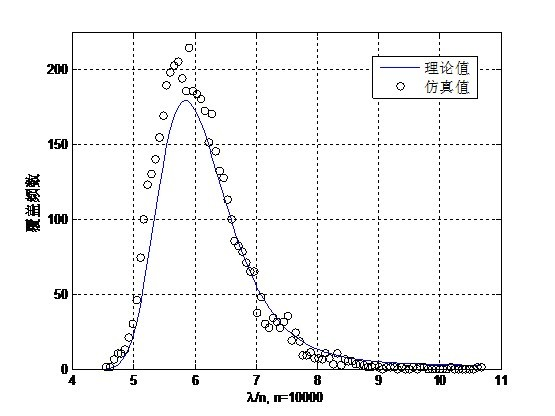
\includegraphics[bb=0 0 410 307,scale=.8]{2.jpg}
\caption{When the network size is $n=10000$, the probability distribution of address space the certification covered.}
\label{fig:f2}
\end{figure}
\begin{figure}[htbp]
\centering
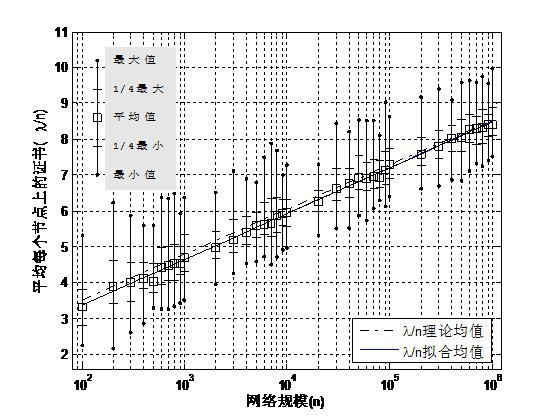
\includegraphics[bb=0 0 410 307,scale=.8]{3.jpg}
\caption{In different network size, the average number of certifications $ \frac{\lambda}{n} $ every node saved.}
\label{fig:f3}
\end{figure}
\begin{equation}
    \frac{\lambda}{n}=1.2792*\lg{n}+0.8103
\end{equation}
You can observed that this linear Fitting is almost close to the mean value of $\frac{\lambda}{n}$. Compared with (19) and (20), you can find that the differences of coefficient of $\lg{n}$ is quite small. And in Figure 3, you can find that the theoretical mean curve calculated by (19) is very similar with the mean curve by (20).  
\section{Conclusion}
In the open networking environment. It is difficult to defense the Sybil Attack.The RM algorithm requires that the number of nodes that the adversaries control can not exceed   of totals. This condition can be easy satisfied. But how to carry out the K-Round replacement scheme in RM algorithm is one barrier in practical application.\\
Considered that the cost of the Byzantine algorithm is expensive, this paper use an explicit CA to handle this problem. By using CA to send the signature and certifications to the joined nodes, this can make sure the node ID can be verified and can not be forged. This certification records one complete k-rounds replacement process. It is the credential to enter the network. In order to prevent the adversaries using the expired ID to join the network by the protocol of topology maintenance. This paper use the replacement intervals of certifications to verify the ID validity. This validity algorithm requires that the contained certifications can completely cover the whole neighbour range, and the key problem is how many certifications is suitable. This paper regard this problem as to cover the circle by random segments. By analysis, we got the approximate solution. The theoretical analysis and simulation experiments show that the average number of certifications to be saved on every node is small, that is  . Then we make sure the scheme is acceptable. 
% Results and Discussion can be combined.
\section*{Results}

\subsection*{Subsection 1}

\subsection*{Subsection 2}

\section*{Discussion}

% You may title this section "Methods" or "Models". 
% "Models" is not a valid title for PLoS ONE authors. However, PLoS ONE
% authors may use "Analysis" 
\section*{Materials and Methods}

% Do NOT remove this, even if you are not including acknowledgments
\section*{Acknowledgments}


%\section*{References}
% The bibtex filename
\bibliographystyle{plain}
\bibliography{template}

\section*{Figure Legends}
%\begin{figure}[!ht]
%\begin{center}
%%\includegraphics[width=4in]{figure_name.2.eps}
%\end{center}
%\caption{
%{\bf Bold the first sentence.}  Rest of figure 2  caption.  Caption 
%should be left justified, as specified by the options to the caption 
%package.
%}
%\label{Figure_label}
%\end{figure}


\section*{Tables}
%\begin{table}[!ht]
%\caption{
%\bf{Table title}}
%\begin{tabular}{|c|c|c|}
%table information
%\end{tabular}
%\begin{flushleft}Table caption
%\end{flushleft}
%\label{tab:label}
% \end{table}

\end{document}

